This chapter will be focusing on defining the needs, selecting the candidates and setting up a test battery that will be used to compare the solutions.

Based on defined criteria, the test battery should be able to provide a fair comparison of the chosen solutions, giving a similar systematic test approach for each one.

The candidate selection, again based on defined criteria, should be able to rank every potential candidate based on an individual mark.

\section{Goals} \label{goals}

This project aims to compare different solutions that make GPU programming available in Java. Our measures will be based on the execution speed and ease of use.

We basically need either Java frameworks that give GPU computing access via some API's or solutions that directly convert Java bytecode so it is runnable on a GPU.

\section{Pre-analysis}

This chapter will be focused on selecting the candidates we want to use for our comparisons. Based on some criteria, we will run through each candidate (see appendix \ref{candidates}) we found and look if they are interesting enough to be chosen. Our criteria  will be :

\begin{itemize}
  \item Time since the last update
  \item Adoption level, community activity and documentation
  \item Adequacy for our needs
\end{itemize}


\subsection{Time since last update}

If available, the time since the last update will be the last commit. If there is no public SVN, repository or possibilities to find the last code commit, we will be looking at the date of the last product release. We will take the most recent date found.

\subsection{Adoption level, community activity and documentation}

For those criteria, mostly subjective, we will be looking at :

\begin{itemize}
  \item Quantity of pertinent search results in Google
  \item Commit activity (if available)
  \item Forum activity (if exists)
  \item Quantity of comments, articles and blogs found
\end{itemize}

\subsection{Adequacy}

For this criteria, we will be looking at the functionalities provided and see if it meets the needs of our project. Basically, it should be able to provide GPU computing capabilities via Java programming.

\newpage

\subsection{Pre-analysis table} \label{pre analysis}

\begin{longtable}{ | p{.15\textwidth} | p{.55\textwidth} | p{.30\textwidth} | }
  
  \hline
  
  \textbf{Time from update} & \textbf{Adoption level, community activity \& documentation} & \textbf{Adequacy} \\
  
  \hline \hline
  
  \multicolumn{3}{|l|}{\textbf{aparapi}} \\

  \hline

  3 months &
  Aparapi, developed by AMD, appears often in articles and researches. Seems to be in a very high adoption level and has a good documentation. &
  Allow GPU programming via bytecode translation for OpenCL. \\
  
  \hline \hline

  \multicolumn{3}{|l|}{\textbf{rootbeer}} \\

  \hline

  9 months &
  According to the readme on Github, it is still in a pre-production beta. It doesn't claim to offer
  a simple GPU programming tool giving an easily high speed up. Was under active development last year but
  seems to be left with no recent updates. It is having its longest time of inactivities since its beginning.
  Documentation not very elaborated. &
  Allow GPU programming by converting bytecode to CUDA programs. \\
  
  \hline \hline
  
  \multicolumn{3}{|l|}{\textbf{java-gpu}} \\

  \hline

  6 years &
  Doesn't seem to be maintained anymore. Has no documentation and no recent version. &
  Allow GPU programming by translating bytecode into CUDA code. \\
  
  \hline \hline
  
  \multicolumn{3}{|l|}{\textbf{ScalaCL}} \\

  \hline

  A year &
  Development stopped a year ago. Not actively maintained, seems to be dying. &
  Offers GPU programming via Scala and not directly with Java. \\
  
  \hline \hline
  
  \multicolumn{3}{|l|}{\textbf{JavaCL}} \\

  \hline

  6 months &
  Has a decent documentation but no recent activities this past years. The activities graph on github seems to show 
  that the project is dying. &
  An OpenCL wrapper for Java. \\
  
  \hline \newpage \hline
  
  \multicolumn{3}{|l|}{\textbf{jocl}} \\

  \hline

  A year &
  It has its own website and forum, which is not actively used (only 1 post this year so far). Doesn't seem
  to have a solid documentation. &
  Java binding 1:1 mapping to OpenCL \\
  
  \hline \hline
  
  \multicolumn{3}{|l|}{\textbf{lwjgl}} \\

  \hline

  today &
  It is a popular framework with a solid documentation and an active forum. &
  This is a game framework that is not primarily suited for GPU programming. \\
  
  \hline \hline
  
  \multicolumn{3}{|l|}{\textbf{jcuda}} \\

  \hline

  Last month &
  Has it's own website and forum, which is not very active. Has some tutorials and an api documentation that seems well. &
  Translate special Java code to CUDA-C. \\
  
  \hline \hline
  
  \multicolumn{3}{|l|}{\textbf{jacc}} \\

  \hline

  This year &
  Is not available and still under development. &
  Java framework that performs on low-level at runtime to use the GPU. \\
  
  \hline \hline
  
  \multicolumn{3}{|l|}{\textbf{CUDA4J}} \\

  \hline

  Last year &
  Is updated to Java 8 and developed by IBM, which certainly means a long time support. &
  Java programming API that uses lambdas and streams. \\
  
  \hline \hline
  
  \multicolumn{3}{|l|}{\textbf{PJ2}} \\

  \hline

  Last month &
  It is an API developed at the Rochester Institute. It is still under maintenance but doesn't have
  a community and is not really well known. &
  Middleware API for Java programming on multicore platforms. \\
  
  \hline

\end{longtable}

\subsection{Grades} \label{grades}

To rank our options, we will give, based on each criteria, a grade going from 0 to 10, 10 being the best and 0 the worst.

Time from update, adoption level and adequacy grade will go according to the following tables:

\begin{center}
\captionof{table}{Grade: Time from update}
\begin{tabular}{|c|c|c|c|c|}
	\hline
	< 3 months & < 6 months & < 1 years & < 2 years & > 2 years \\
	\hline
	10 & 8 & 5 & 3 & 0 \\
	\hline
\end{tabular}
\end{center}

\begin{center}
\captionof{table}{Grade: Adoption level, community activity and documentation}
\begin{tabular}{|p{.25\textwidth}|p{.25\textwidth}|p{.25\textwidth}|p{.25\textwidth}|}
	\hline
	Is well referenced, found many articles and is well documented & 
	Appears quite often in a google search, found some articles and has a fairly good documentation &
	Found some results in a google search and has a documentation &
	Didn't found much results in a google search, has a poor documentation \\
	\hline
	10 & 8 & 5 & 3 \\
	\hline
\end{tabular}
\end{center}

\begin{center}
\captionof{table}{Grade: Adequacy}
\begin{tabular}{|p{.25\textwidth}|p{.25\textwidth}|p{.25\textwidth}|p{.25\textwidth}|}
	\hline
	Fits perfectly our needs & 
	Fits partially our needs, or the solution is not aimed to particularly fits out needs &
	Doesn't fit our needs \\
	\hline
	10 & 3 & 0 \\
	\hline
\end{tabular}
\end{center}

\subsection{Grades table}

According to our pre-analysis (see section \ref{pre analysis}) and our grades (section \ref{grades}), each candidates has been evaluated and got a corresponding mark. Based on the marks, we will choose the candidates that have the highest ones.

\begin{longtable}{ | p{.20\textwidth} | p{.20\textwidth} | p{.20\textwidth} | p{.20\textwidth} | p{.10\textwidth} | }
  
  \hline
  
  & Time from update & Adoption level, community activity \& documenation & Adequacy & \textbf{Grade} \\
  
  \hline \hline
  
  \textbf{aparapi} &
  10 &
  10 &
  10 &
  \textbf{30} \\
  
  \hline \hline
  
  \textbf{jcuda} &
  10 &
  8 &
  10 &
  \textbf{28} \\
  
  \hline \hline
  
  \textbf{CUDA4J} &
  5 &
  10 &
  10 &
  \textbf{25} \\
  
  \hline \hline
 
  \textbf{PJ2} &
  10 &
  5 &
  10 &
  \textbf{25} \\
  
  \hline \hline

  \textbf{rootbeer} &
  5 &
  8 &
  10 & 
  \textbf{23} \\
  
  \hline \hline
  
  \textbf{java-gpu} &
  8 &
  5 &
  10 &
  \textbf{23} \\
  
  \hline \hline
  
  \textbf{JavaCL} &
  8 &
  5 &
  10 &
  \textbf{23} \\
  
  \hline \hline
  
  \textbf{lwjgl} &
  10 &
  10 &
  3 &
  \textbf{23} \\
  
  \hline \hline
  
  \textbf{jacc} &
  5 &
  5 &
  10 &
  \textbf{20} \\
  
  \hline \hline
  
  \textbf{jocl} &
  5 &
  5 &
  10 &
  20 \\
  
  \hline \hline
  
  \textbf{ScalaCL} &
  5 &
  5 &
  10 &
  20 \\
  
  \hline

\end{longtable}

\section{Nominees}

Based on our prior analysis, we will only be focusing on the first two technologies, which obtained the highest grades with 30/30 for Aparapi and 28/30 for JCuda. Those technologies will give us the opportunity to test an openCL and CUDA based solution.


\section{Battery of tests} \label{battery test}

Testing our solution will require us to write a first implementation using vanilla Java code, then writing two other implementations - still in Java - but adapted to use a specific solution (in our case, it will be Aparapi and JCuda). We will then be able to compare the implementations.

We will base our tests on two main aspects :

\begin{enumerate}
  \item Speed
  \item Ease of use
\end{enumerate}

\textbf{1: The first aspect - Speed -} will use some benchmarks code testing specific computation aspects like floating point operations or integer manipulations. Those tests will give us precise metrics that will be easily comparable.

\textbf{2: The second aspect - ease of use -} are more kind of subjective and will need a systematic approach so as to be the most fair. We will be looking at some defined criteria, like the number of code lines and the programmer's feedback. The next section will discuse in more details the two aspects.

\subsection{Speed} \label{subsection speed}

To add more relevance to our benchmark, we wanted to choose two benchmarks that does not perform the same type of operations. The most obvious one - a matrix computation - was our first choice. Due to its simple implementation and its ability to be distributed on different cores, we rapidly opted for this one. The matrix multiplication will be able to measure floating point manipulations performance. 

Our second choice was to make an array sorting. But, after testing some pieces of code, we went back and looked for another alternative. The idea of the array sorting, as shown in figure \ref{fig sort}, was to split the array, distribute the subsets and perform a merge sort. This solution was simple to code but performed very badly concerning memory space.

\begin{figure}[h!]
\centering
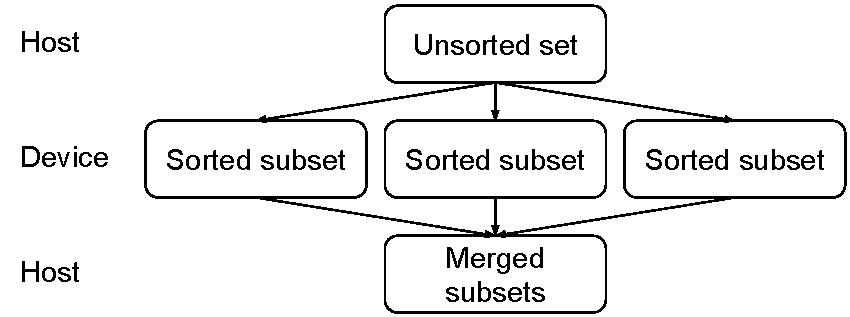
\includegraphics[width=0.7\textwidth]{sort}
\caption{Sorting principle}
\label{fig sort}
\end{figure}

We then looked for the prime factorization of an integer. Again, quite easy to code (see figure \ref{listing factor}), but this time our implementation wasn't suited to be ported on a multi-threaded architecture and was highly limited by Java integer size, even using \textit{BigInteger}.

\begin{figure}
	\begin{lstlisting}
BigInteger n = 999999;
BigInteger i = new BigInteger("2");
for(; i.compareTo(n.divide(i)) <= 0; i = i.add(BigInteger.ONE)) {
  while(n.mod(i).equals(BigInteger.ZERO)) {
    System.out.println("Divisor: " + n);
    n = n.divide(i);
  }
}
	\end{lstlisting}
\caption{Factorization of a number}
\label{listing factor}
\end{figure}

We finally opted for the computation of a Levenshtein distance between two strings. The code remains simple, is not heavily restrained by variables' size and can be adapted to a multi-threaded architecture.

To summarize, the speed measure will be based on those two simple computation operations :

\begin{enumerate}
  \item A matrix multiplication using floating variables
  \item Levenshtein distance computation of two strings
\end{enumerate}

\textbf{1: The matrix multiplication} will be as simple as possible, using the basic definition saying that each cell of the resulting matrix $C {{=}} AB$ is given by the following formula :

\begin{equation}
	c_{ij} = \sum_{k=1}^m a_{ik} b_{kj}
\end{equation}

This method leads to a complexity of $O(n^3)$ for a squared matrix of size $n$, which is fine for a benchmark purpose. To have a code as flexible as possible, we won't use any Java matrix objects, but only 2-dimensions doubles arrays. figure \ref{listing matrix} shows a sample code of the matrix multiplication.

\begin{figure}[h!]
\begin{lstlisting}
  // Computes matrix multiplication C = AB
  public static void matrixMul(double[][] A, double[][] B, 
                               double[][] C) {
    for(int i=0; i < size; i++) {
      for(int j=0; j < size; j++) {
        double sum = 0.0;
        for(int k=0; k < size; k++) {
          sum += A[i][k] * B[k][j];
        }
        C[i][j] = sum;
      }
    }
  }
\end{lstlisting}
\caption{Sample code of the matrix multiplication}
\label{listing matrix}
\end{figure}

Adapting the code on a multithreaded architecture won't be difficult since each cell, row or column can be computed independently on a separate core.

The matrix content will be randomized and adjusted according to the matrix size so as to prevent overflows. The size will be set to produce a computation time from 30 seconds to 1 minute. The random seed will be the same among all our tests so as to keep the same conditions.

Figure \ref{fig plot matrix} is a quick single measure of the complexity scale of our implementation. The result has been compared to other same measures so as to ensure that there is no edge cases or noise in our results. Raw values of this measure are available in the appendix \ref{raw values quick matrix}, and the comparison made with another measure can be found in the appendix \ref{vanilla matrix both}.

\begin{figure}[h!]
\centering
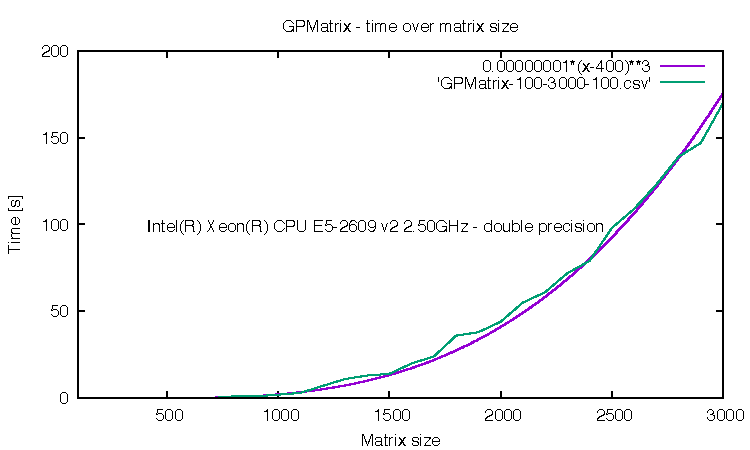
\includegraphics[width=1\textwidth]{vanillaPlotMatrix}
\caption{Complexity scale of the matrix implementation}
\label{fig plot matrix}
\end{figure}


\textbf{2: The Levenshtein distance} will be based on the definition found on wikipedia\cite{levenshteinwiki} stating that:

$\qquad\operatorname{lev}_{a,b}(i,j) = \begin{cases}
  \max(i,j) & \text{ if} \min(i,j)=0, \\
  \min \begin{cases}
          \operatorname{lev}_{a,b}(i-1,j) + 1 \\
          \operatorname{lev}_{a,b}(i,j-1) + 1 \\
          \operatorname{lev}_{a,b}(i-1,j-1) + 1_{(a_i \neq b_j)}
       \end{cases} & \text{ otherwise.}
\end{cases}$

 We will use an already existing implementation\cite{levenshtein} that will be adapted for a multi-threaded use.
The strings will be generated randomly and the size will be adjusted to give a computation time from 30 seconds to 1 minute. The strings will be stored in files. It has the advantages of being reusable and not limited by the maximum Java string size or input parameter size. The listing \ref{listing leven} is a sample code computing the Levenstein distance. This is the one that will be adapted to be used on the GPU.

\begin{figure}[h!]
\begin{lstlisting}
  public static int distance(String a, String b) {
    int [] costs = new int [b.length() + 1];
    for (int j = 0; j < costs.length; j++)
      costs[j] = j;
    for (int i = 1; i <= a.length(); i++) {
      costs[0] = i;
      computeRow(costs, i, a, b);
    }
    return costs[b.length()];
  }

  // Compute a single row in the distance process
  public static void computeRow(int[] costs, int i, String a, String b) {
    int nw = i - 1;
    for (int j = 1; j <= b.length(); j++) {
      int cj = Math.min(1 + Math.min(costs[j], costs[j - 1]), a.charAt(i - 1) == b.charAt(j - 1) ? nw : nw + 1);
      nw = costs[j];
      costs[j] = cj;
    }
  }
\end{lstlisting}
\caption{Sample code of the Levenstein distance computation}
\label{listing leven}
\end{figure}


Figure \ref{fig plot leven} is a measure of the complexity scale of the implementation. We took an average based on 5 executions. In this case, we observe a complexity of $O(n^2)$, which grows much less than the matrix multiplication. Raw values of this measure can be found in the appendix \ref{raw values quick leven}.

\begin{figure}[h!]
\centering
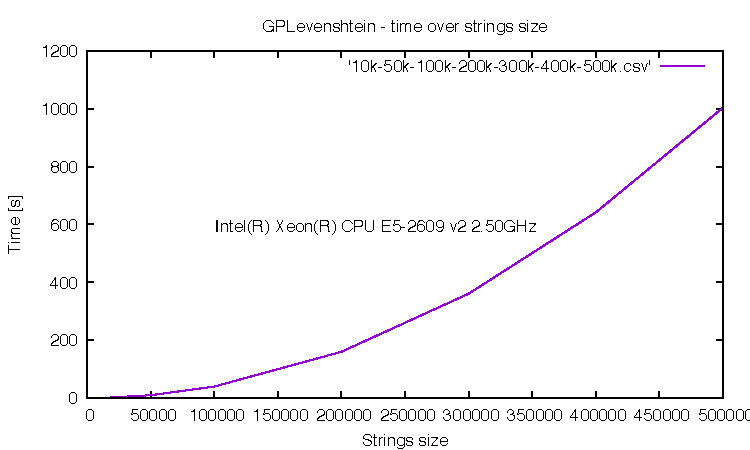
\includegraphics[width=1\textwidth]{vanillaPlotLeven2}
\caption{Complexity scale of the Levenshtein implementation, average on 5 executions}
\label{fig plot leven}
\end{figure}

\subsection{Ease of use}

To measure the ease of use, we will be looking at :

\begin{enumerate}
  \item The number of line codes (LOC)
  \item A personal feedback after the solution's installation
  \item External reviews of the code by some developers
  \item A personal feedback after the execution of the test battery
\end{enumerate}

\textbf{1: The line of codes} will be taken from the routines performing the speed tests mentioned in the previous subsection (\ref{subsection speed}). Each routine will be evaluated separately and compared to the other implementations. We won't take blank lines and comments into account.

\textbf{2: The personal feedback} will be written right after the setting up of the solution. This feedback will evaluate if the solution is hard to set up or easily usable, like an out-of-the box solution. The environment will already have CUDA and OpenCL set up, so that part will not be evaluated.

\textbf{3: Having an external review} from some developers will help having a fresh point of view. While developing and judging his own code can alter an opinion, someone external will have a neat more objective point of view concerning the complexity of a code. Those persons will be asked to understand the code and give a grade from 1 (very hard) to 5 (very easy) about how it is hard or not to understand how the code uses the GPU.

\textbf{4: The personal conclusion} will be a conclusion after the end of the test battery. It will give an overall feedback about the setting up and development with a particular solution.

\subsection{Test process}

Figure \ref{fig tprocess} shows the sequential process that will be applied for our test battery.

\begin{figure}[h!]
\centering
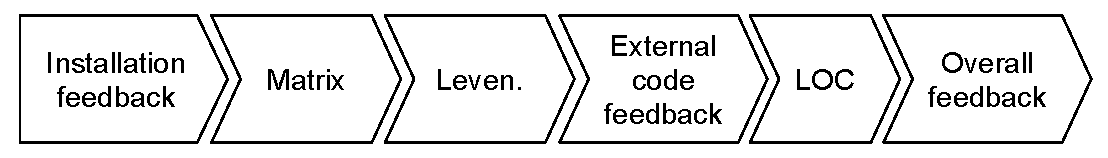
\includegraphics[width=1\textwidth]{testprocess}
\caption{Testing process}
\label{fig tprocess}
\end{figure}